\documentclass[12pt]{article}

\usepackage{fontspec}
\newfontfamily\handwriting{a-casual-handwritten-pen}[Path=../assets/fonts/,Extension=.ttf,Scale=1.5]
\newfontfamily\comic{Comic Neue}

\usepackage[utf8]{inputenc}
\usepackage{amsmath}
\usepackage{amssymb}
\usepackage{enumitem}
\usepackage{xcolor}
\usepackage{soul}
\usepackage{tikz}
\usepackage[most]{tcolorbox}
\usepackage{titlesec}
\usepackage{multicol}
\usepackage{environ}

\usetikzlibrary{fit, positioning, arrows.meta}

% --- Custom Colors ---
\definecolor{primaryblue}{RGB}{42, 111, 151}
\definecolor{exbg}{RGB}{255, 240, 245}
\definecolor{rulebg}{RGB}{232, 245, 233}
\definecolor{highlight}{RGB}{255, 243, 176}
\definecolor{pinkanno}{RGB}{255, 105, 180}
\definecolor{purpleanno}{RGB}{147, 112, 219}
\definecolor{solutionbg}{RGB}{245, 245, 255}

% --- Header Styling ---
\titleformat{\section}{\color{primaryblue}\normalfont\Large\bfseries}{\thesection}{1em}{}
\titleformat{\subsection}{\color{primaryblue}\normalfont\large\bfseries}{\thesubsection}{1em}{}

% --- Friendly Boxes ---
% --- Auto-numbered Example Box ---
\newcounter{examplenum}

\newtcolorbox{friendlyexbox}[1]{
    colback=exbg,
    colframe=pinkanno!50,
    arc=5pt,
    title=\textbf{#1},
    coltitle=black,
    attach title to upper,
    after title={:\quad}
}

\newenvironment{friendlyex}{%
    \refstepcounter{examplenum}%
    \begin{friendlyexbox}{Example \theexamplenum}%
}{%
    \end{friendlyexbox}%
}

\newtcolorbox{friendlyrule}[1]{
    colback=rulebg,
    colframe=primaryblue!30,
    arc=5pt,
    fonttitle=\bfseries,
    title={#1},
    coltitle=primaryblue
}

\newcommand{\funhl}[1]{\sethlcolor{highlight}\hl{#1}}

% --- Show/Hide Solutions ---
\newif\ifshowsolutions

% Uncomment the next line to show solutions.
\showsolutionstrue

\newcommand{\solutionblank}{\vspace{25ex}}

\NewEnviron{solutionbox}{
\ifshowsolutions
\begin{tcolorbox}[
    colback=solutionbg,
    colframe=purpleanno!45,
    arc=5pt,
    title={Solution},
    coltitle=primaryblue,
    fonttitle=\bfseries
]
\BODY
\end{tcolorbox}
\else
\solutionblank
\fi
}

\begin{document}
\handwriting

\begin{center}
    \Large\textbf{\color{primaryblue}Module 1 Lesson 1\\Function and Function Notation} \\
    \vspace{0.2cm}
    \hrule
\end{center}

\section*{Objectives}

\begin{friendlyrule}{In this lesson, we will learn how to}
\begin{itemize}
    \item define a relation and identify its domain and range;
    \item decide whether a relation is a function;
    \item use the vertical line test;
    \item find $x$- and $y$-intercepts using function notation;
    \item evaluate a function at a given input.
\end{itemize}
\end{friendlyrule}

\section*{1. Relations, Domain, and Range}

A \funhl{relation} in $x$ and $y$ is a set of ordered pairs $(x,y)$.

\begin{friendlyrule}{Domain and Range}
\begin{itemize}
    \item The set of $x$-values in the ordered pairs is called the \funhl{domain} of the relation.
    \item The set of $y$-values in the ordered pairs is called the \funhl{range} of the relation.
\end{itemize}
\end{friendlyrule}

\section*{2. Functions}

Given a relation in $x$ and $y$, we say that $y$ is a \funhl{function} of $x$ if for each value of $x$ in the domain, there is exactly one value of $y$ in the range.

Example of a function: \\

\[
\text{Domain}=\{1,2,5,7\}\qquad(\text{independent variables, }x\text{'s}),
\]
\[
\text{Range}=\{4,6,-3,10\}\qquad(\text{dependent variables, }y\text{'s}),
\]

paired as shown below:

\begin{center}
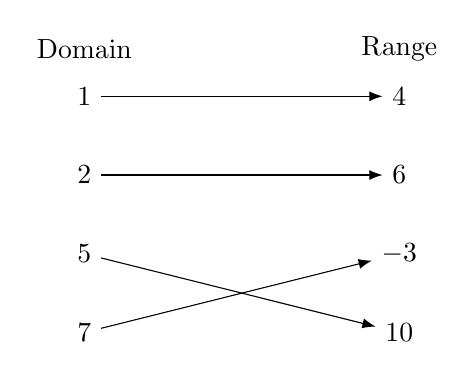
\begin{tikzpicture}[scale=1, every node/.style={font=\handwriting}]
\node at (0,3.6) {Domain};
\node at (4,3.6) {Range};
\node (x1) at (0,3) {$1$};
\node (x2) at (0,2) {$2$};
\node (x3) at (0,1) {$5$};
\node (x4) at (0,0) {$7$};
\node (y1) at (4,3) {$4$};
\node (y2) at (4,2) {$6$};
\node (y3) at (4,1) {$-3$};
\node (y4) at (4,0) {$10$};
\draw[-{Latex}] (x1) -- (y1);
\draw[-{Latex}] (x2) -- (y2);
\draw[-{Latex}] (x3) -- (y4);
\draw[-{Latex}] (x4) -- (y3);
\end{tikzpicture}
\end{center}

\begin{friendlyex}
Consider the domain and range

\[
\text{Domain}=\{1,2,5,7\}\qquad(\text{independent variables, }x\text{'s}),
\]

\[
\text{Range}=\{4,6,-3,10\}\qquad(\text{dependent variables, }y\text{'s}),
\]

paired as shown below:

\begin{center}
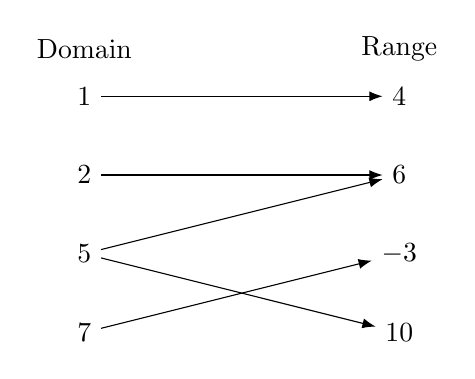
\begin{tikzpicture}[scale=1, every node/.style={font=\handwriting}]
\node at (0,3.6) {Domain};
\node at (4,3.6) {Range};
\node (x1) at (0,3) {$1$};
\node (x2) at (0,2) {$2$};
\node (x3) at (0,1) {$5$};
\node (x4) at (0,0) {$7$};
\node (y1) at (4,3) {$4$};
\node (y2) at (4,2) {$6$};
\node (y3) at (4,1) {$-3$};
\node (y4) at (4,0) {$10$};
\draw[-{Latex}] (x1) -- (y1);
\draw[-{Latex}] (x2) -- (y2);
\draw[-{Latex}] (x3) -- (y2);
\draw[-{Latex}] (x3) -- (y4);
\draw[-{Latex}] (x4) -- (y3);
\end{tikzpicture}
\end{center}

This gives the ordered pairs

\[
(1,4),\qquad (2,6),\qquad (5,6),\qquad (7,-3),\qquad (5,10).
\]

Is this a function?
\end{friendlyex}

 

\begin{solutionbox}
Look at the $x$-value $5$. It is paired with both $6$ and $10$:

\[
(5,6)\qquad\text{and}\qquad (5,10).
\]

One $x$ cannot be paired with more than one $y$.

Therefore, this relation is \textbf{not} a function.

\emph{Note:} it is perfectly fine for one $y$-value to be paired with more than one $x$-value --- notice $6$ is paired with both $2$ and $5$ above, and that alone does not break the function rule.
\end{solutionbox}

  

\begin{friendlyex}
Consider pairing players on a basketball team with their heights:

\begin{center}
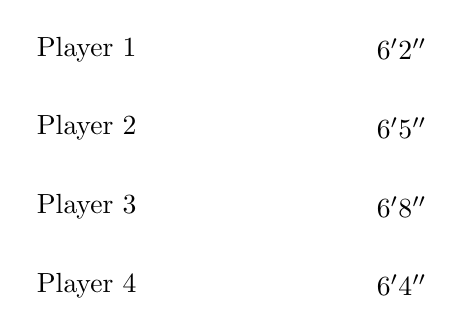
\begin{tikzpicture}[scale=1, every node/.style={font=\handwriting}]
\node (x1) at (0,3) {Player 1};
\node (x2) at (0,2) {Player 2};
\node (x3) at (0,1) {Player 3};
\node (x4) at (0,0) {Player 4};
\node (y1) at (4,3) {$6'2''$};
\node (y2) at (4,2) {$6'5''$};
\node (y3) at (4,1) {$6'8''$};
\node (y4) at (4,0) {$6'4''$};
\end{tikzpicture}
\end{center}

If this relation were not a function, what would have to happen?
\end{friendlyex}

 

\begin{solutionbox}
As given, every player is paired with exactly one height, so this relation \textbf{is} a function.

For it to fail to be a function, some player would have to be paired with two different heights --- for example, if Player 1 were listed as both $6'2''$ and $6'5''$.
\end{solutionbox}

  

\section*{3. The Vertical Line Test}

\begin{friendlyrule}{Vertical Line Test}
A graph represents a function if and only if no vertical line intersects the graph at more than one point.
\end{friendlyrule}

\begin{friendlyex}
Does each graph below represent a function?

\begin{center}
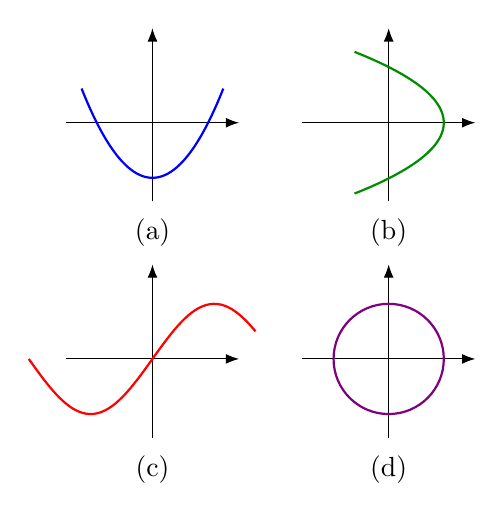
\begin{tikzpicture}[scale=0.5]
% panel (a): upward parabola -- function
\begin{scope}[shift={(0,0)}]
\draw[-{Latex}] (-2.2,0) -- (2.2,0);
\draw[-{Latex}] (0,-2) -- (0,2.4);
\draw[blue, thick, domain=-1.8:1.8, samples=50, smooth] plot (\x, {0.7*\x*\x - 1.4});
\node at (0,-2.8) {(a)};
\end{scope}
% panel (b): sideways parabola -- not a function
\begin{scope}[shift={(6,0)}]
\draw[-{Latex}] (-2.2,0) -- (2.2,0);
\draw[-{Latex}] (0,-2) -- (0,2.4);
\draw[green!55!black, thick, domain=-1.8:1.8, samples=50, smooth] plot ({1.4 - 0.7*\x*\x}, \x);
\node at (0,-2.8) {(b)};
\end{scope}
% panel (c): wave -- function
\begin{scope}[shift={(0,-6)}]
\draw[-{Latex}] (-2.2,0) -- (2.2,0);
\draw[-{Latex}] (0,-2) -- (0,2.4);
\draw[red, thick, domain=-180:150, samples=60, smooth] plot ({\x/57.3}, {1.4*sin(\x)});
\node at (0,-2.8) {(c)};
\end{scope}
% panel (d): circle -- not a function
\begin{scope}[shift={(6,-6)}]
\draw[-{Latex}] (-2.2,0) -- (2.2,0);
\draw[-{Latex}] (0,-2) -- (0,2.4);
\draw[violet, thick] (0,0) circle (1.4);
\node at (0,-2.8) {(d)};
\end{scope}
\end{tikzpicture}
\end{center}
\end{friendlyex}

 

\begin{solutionbox}
\begin{itemize}
    \item[(a)] \textbf{Function.} Every vertical line crosses the upward-opening parabola exactly once.
    \item[(b)] \textbf{Not a function.} A vertical line through the middle of the sideways parabola crosses it twice.
    \item[(c)] \textbf{Function.} Every vertical line crosses the wave exactly once.
    \item[(d)] \textbf{Not a function.} A vertical line through the interior of the circle crosses it twice.
\end{itemize}
\end{solutionbox}

  

\begin{friendlyex}
Consider the table

\[
\begin{array}{c|cccc}
x & -1 & 6 & \, & 5 \\ \hline
y & 12 & 8 & -5 & 4
\end{array}
\]

If this table were \emph{not} a function, what would have to happen?
\end{friendlyex}

 

\begin{solutionbox}
For the table to fail to represent a function, some $x$-value would need to appear twice with two different $y$-values --- for instance, if $x=6$ were paired with both $8$ and $-5$.
\end{solutionbox}

  

\section*{4. Finding $x$- and $y$-Intercepts Using Function Notation}

\begin{friendlyrule}{Intercepts from $y=f(x)$}
\begin{itemize}
    \item The \funhl{$x$-intercepts} are the real solutions of $f(x)=0$. They are the points where the graph crosses the $x$-axis.
    \item The \funhl{$y$-intercept} is given by $f(0)$. It is the point where the graph crosses the $y$-axis.
\end{itemize}
\end{friendlyrule}

\begin{friendlyex}
Find the $x$- and $y$-intercepts of

\[
\text{(i)}\quad f(x)=4x-12, \qquad\qquad \text{(ii)}\quad f(x)=x^2-25.
\]
\end{friendlyex}

 

\begin{solutionbox}
\textbf{(i)} Set $f(x)=0$:

\[
4x-12=0\ \Longrightarrow\ x=3.
\]

The $x$-intercept is $(3,0)$.

The $y$-intercept is

\[
f(0)=4(0)-12=-12,
\]

so the $y$-intercept is $(0,-12)$.

\textbf{(ii)} Set $f(x)=0$:

\[
x^2-25=0\ \Longrightarrow\ x^2=25\ \Longrightarrow\ x=\pm 5.
\]

The $x$-intercepts are $(5,0)$ and $(-5,0)$.

The $y$-intercept is

\[
f(0)=0^2-25=-25,
\]

so the $y$-intercept is $(0,-25)$.
\end{solutionbox}

  

\section*{5. Function Notation: Naming the Rule}

One of the most common ways to represent a function is by a formula or rule. For example,

\[
f(x)=x^2+1\qquad\text{or}\qquad y=x^2+1.
\]

The function's name is $f$. Its rule says: ``to find the number that $x$ is paired with, you square $x$ and then add $1$ to the result.''

\section*{6. Evaluating Functions}

\begin{friendlyex}
Evaluate each function at the given input.

\begin{itemize}
    \item[(a)] If $G(x)=3x^3-x-2$, find $G(2)$.
    \item[(b)] If $p(r)=\sqrt{r^2+7}-2$, find $p(-3)$.
    \item[(c)] If $r(s)=\dfrac{4-s}{2+s}$, find $r(-2)$.
    \item[(d)] Let $f(x)=\sqrt{x-4}$. Determine $x$ for which $f(x)=3$.
\end{itemize}
\end{friendlyex}

 

\begin{solutionbox}
\textbf{(a)}

\[
G(2)=3(2)^3-2-2=3(8)-4=24-4=20.
\]

\textbf{(b)}

\[
p(-3)=\sqrt{(-3)^2+7}-2=\sqrt{9+7}-2=\sqrt{16}-2=4-2=2.
\]

\textbf{(c)} Substituting $s=-2$ gives

\[
r(-2)=\frac{4-(-2)}{2+(-2)}=\frac{6}{0}.
\]

Since we cannot divide by zero, $r(-2)$ is \textbf{undefined}. (This is a preview of \emph{domain} --- see the next lesson!)

\textbf{(d)}

\[
\sqrt{x-4}=3\ \Longrightarrow\ x-4=9\ \Longrightarrow\ x=13.
\]
\end{solutionbox}

  

\section*{7. More Practice with Function Notation}

\begin{friendlyex}
Given the table representing a function $f$,

\[
\begin{array}{c|cccccc}
x & -2 & -1 & 3 & 4 & 6 & 10 \\ \hline
f(x) & 4 & 8 & 0 & -2 & 8 & 5
\end{array}
\]

\begin{itemize}
    \item[(a)] Determine $f(4)$.
    \item[(b)] Solve $f(x)=8$ for $x$.
\end{itemize}
\end{friendlyex}

 

\begin{solutionbox}
\textbf{(a)} Reading the table at $x=4$:

\[
f(4)=-2.
\]

\textbf{(b)} We look for $x$-values whose output is $8$. Both $x=-1$ and $x=6$ give output $8$, so

\[
x=-1\qquad\text{or}\qquad x=6.
\]
\end{solutionbox}

  

\begin{friendlyex}
If a rock falls from a height of $100$ meters on a planet $P$, its height $H$ (in meters) after $t$ seconds is approximately

\[
H(t)=100-3t^2.
\]

\begin{itemize}
    \item[(a)] What is the height of the rock when $t=1$, $t=2$, and $t=3$?
    \item[(b)] When is the height of the rock $52$ meters?
\end{itemize}
\end{friendlyex}

 

\begin{solutionbox}
\textbf{(a)}

\[
H(1)=100-3(1)^2=97,
\]

\[
H(2)=100-3(2)^2=100-12=88,
\]

\[
H(3)=100-3(3)^2=100-27=73.
\]

\textbf{(b)} Set $H(t)=52$:

\[
100-3t^2=52.
\]

\[
48=3t^2.
\]

\[
t^2=16.
\]

\[
t=\pm 4.
\]

Since time cannot be negative, we reject $t=-4$. The rock is at $52$ meters when

\[
t=4\text{ seconds.}
\]
\end{solutionbox}

  

\section*{Summary}

\begin{friendlyrule}{Key Ideas}
\begin{itemize}
    \item A relation is a set of ordered pairs $(x,y)$; its domain is the set of $x$-values and its range is the set of $y$-values.
    \item A relation is a function if every $x$-value in the domain corresponds to exactly one $y$-value. It is fine for a $y$-value to repeat.
    \item The vertical line test: a graph is a function if and only if no vertical line crosses it more than once.
    \item The $x$-intercepts of $y=f(x)$ solve $f(x)=0$; the $y$-intercept is $f(0)$.
    \item To evaluate a function, substitute the given input for the variable and simplify.
\end{itemize}
\end{friendlyrule}

\end{document}
